\newpage
\section{Aufbau der Architektur Android App}
\index{Architektur}
\label{sec:Architektur}

Wie bereits erw�hnt werden Android Applikationen in Java geschrieben. Sind grundlegende Java Programmierkenntnisse vorhanden, sollte der Einstieg kein Problem sein. Eine Grundlegende �nderung gilt es jedoch zu beachten:

\begin{itemize}
\item Fast alle Java-Klassen stehen zur Verf�gung plus Verschl�sselung, HTTP, JSON, XML Bibliotheken
\item Es existiert keine main()-Funktion wie bei klassischen Java-Applikationen\\
Es existieren stattdessen lose gekoppelte Komponenten. Eine oder mehrere davon werden als Einstiegspunkt - �hnlich wie main()-Methode - definiert.
\item Die wichtigste Komponente ist die Activity: Sie entspricht einem sichtbaren Fenster auf dem Screen
\end{itemize}

Quelle: \cite{android_architektur}


%-----------------------------------------------------------------------------------------------------------------------------------
\subsection{Activity, View, Event, Intent}
\label{sec:fourElements}
\index{Activity} \index{View} \index{Event} \index{Intent}
Diese vier Begriffe sind die Grundsteine der Android Applikations-Entwicklung.\\
Anbei kurz die wichtigsten Eigenschaften:\\

\textbf{Activity}
\begin{itemize}
\item definiert eine View, zur Anzeige auf dem Screen
\item behandelt Events z. B. Klick auf einen Button - onClick()
\item benutzt Intents, um andere Activities zu starten
\end{itemize}

\textbf{View}
\begin{itemize}
\item die View ist der sichtbare Teil - sie wird auf dem Screen angezeigt wird
\item ist definiert in einer XML-Layout-Datei (oder im Code)
\end{itemize}

\textbf{Event}
\begin{itemize}
\item Wird ausgel�st, wenn etwas geschieht (z. B ein Button geklickt wird)
\item ruft eine Listener-Methode auf, sofern ein Listener definiert ist
\end{itemize}

\textbf{Intent}
\begin{itemize}
\item startet eine andere Activity - �ffnet ein neues Fenster
\item kann Daten an die zu startende Activity �bergeben
\item kann Activities aus anderen Apps starten!
\end{itemize}

%-----------------------------------------------------------------------------------------------------------------------------------
\subsection{Lifecycle Activity}
\label{sec:Lifecycle_Activity}
\index{Lifecycle Activity|see{Activity}} \index{Activity}
Obwohl die Rechenleistungen und der Speicherplatz in den letzten Jahren bei Smartphones rasant angestiegen ist, ist der Speicherplatz im Vergleich zu Workstations noch immer sehr begrenzt. Aus diesem Grund muss das Android-Betriebssystem nicht aktivierte Activities - also diejenigen, die nicht sichtbar sind - beenden k�nnen. Jeder Activity stehen gem�ss folgender Grafik die verschiedenen Zust�nde zur Verf�gung. Auf die Details der einzelnen Zust�nde wird hier verzichtet.\\

\begin{figure}[h!]
\centering
\noindent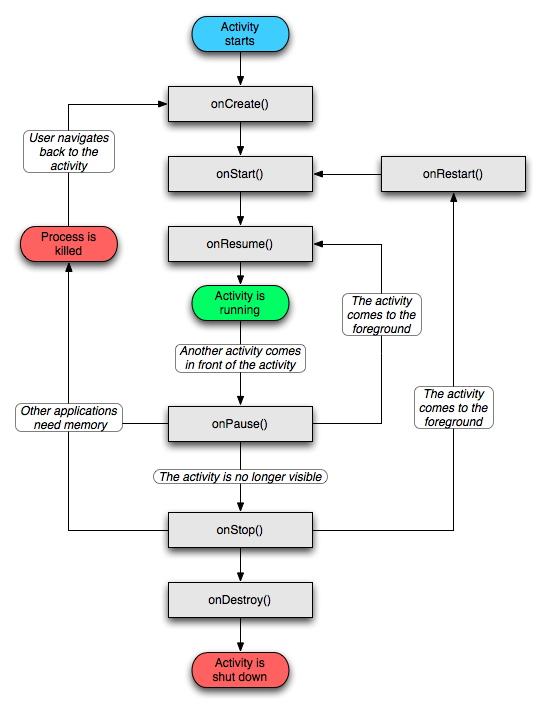
\includegraphics[height=0.65\textheight]{Activity_Lifecycle.png} 
\caption{Lifescyle Activity}
\label{Lifescyle_Activity}
\end{figure}


Quelle: (Kapitel \ref{sec:fourElements} und \ref{sec:Lifecycle_Activity}): \cite{android_architektur}
%-----------------------------------------------------------------------------------------------------------------------------------

\newpage
\subsection{R.java}
\index{R.java} \index{Main Activity}
R.java ist eine selbstgenerierte Java Klasse.
Sie speichert f�r jede Ressource eine Integer-Konstante. F�r die Applikationsentwicklung ist es nicht notwendig, diese Datei einzusehen.
Anbei ein Ausschnitt der R.java Datei unser Applikation.
\lstset{language=Java, numbers=left}
\lstinputlisting[label=lst:latex.listing,captionpos=b, caption=R.java]{dir/03-GrundlagenAppProgrammierung/02-AufbauArchitektur/R.java}
F�r die anderen Klassen hat R.java jedoch eine sehr grosse Bedeutung: Da allen Ressourcen in R.java eine konstante Integer-Variable zugewiesen ist, hat jede *.java Klasse einen Verweis auf R.java, damit das richtige Layout geladen werden kann. Anbei ein Auszug aus MainActivity.java. Diese Activity ist die erste Activity, die geladen wird. Sie ist verkn�pft mit dem Layout \textbf{activity\_main}.

\lstset{language=Java, numbers=left}
\lstinputlisting[label=lst:latex.listing,captionpos=b, caption=MainActivity.java]{dir/03-GrundlagenAppProgrammierung/02-AufbauArchitektur/MainActivity.java}



%-----------------------------------------------------------------------------------------------------------------------------------
\newpage
\subsection{strings.xml}
\index{strings.xml} \index{values} \index{Sprachen}
Die Datei \textbf{strings.xml} wird verwendet, um alle sichtbaren Texte, welche zur Laufzeit der App auf dem Bildschirm erscheinen, zu verwalten.\\
Als Programmierer sollte beachtet werden, dass eine Beschriftung eines Buttons nicht hardcoded wird, da die Flexibilit�t und die lose Kopplung verloren gehen. Wird stattdessen auf die Variable in der strings.xml Datei verwiesen, k�nnen alle App-Texte zentral verwaltet werden.\\
Ist dies einmal gegeben, ist ein Hinzuf�gen einer weiteren Sprache kein Problem mehr.
Defaultm�ssig liegt die strings.xml Datei im Verzeichnis ../res/values/strings.xml und definiert die englische Sprache.\\
M�chte man nun eine weitere Sprache hinzuf�gen, erstellt man f�r die entsprechende Sprache einen neuen Ordner (Beispiel: ../res/\textbf{values-de}/). Nun kann die Datei strings.xml aus ../res/values/ kopiert werden und die Englischen Texte auf Deutsch angepasst werden.\\

Es gibt zwei Varianten, die Sprache der App zu �ndern:
\begin{itemize}
\item Wird nichts eingestellt, wird die App in der Sprache gestartet, welche die Landeseinstellungen des Android Smartphone vorgeben. Ist die entsprechende Sprache in der App nicht vorhanden, wird per default Englisch benutzt.
\item In der App kann ein Menupunkt eingebaut werden, �ber welchen man auf jede beliebige Sprache, welche die App beherrscht, umstellen kann. 
\end{itemize}
\lstset{language=XML, morekeywords={encoding,xs:schema,xs:element,xs:complexType,xs:sequence,xs:attribute}}
\lstinputlisting[label=lst:latex.listing,captionpos=b, caption=strings.xml]{dir/03-GrundlagenAppProgrammierung/02-AufbauArchitektur/strings.xml}



%-----------------------------------------------------------------------------------------------------------------------------------
\newpage
\subsection{Manifest.xml}
\index{Manifest.xml}
Die Datei \textbf{Manifest.xml} ist gewissermassen das Herzst�ck der App. Sie enth�lt die wichtigsten Informationen �ber die App \cite{uni-dortmund}:
\begin{itemize}
\item enth�lt wichtige Informationen, damit die App auf einem System ausf�hrbar ist
\item Manifestdatei enth�lt Metadaten einer App (Paketname)
\item Angabe genutzter Komponenten \\ Aktivities, Services, Broadcast Receivers, Content Providers
\item F�higkeiten der App
\item Voraussetzungen zum Betrieb \\ z.B. n�tige Bibliotheken
\item Intent-Filter und IntentReceiver der Activities
\item Zugriffsrechte auf andere Dienste und Rechte, die andere Apps f�r den Zugriff haben m�ssen
\item Angabe von Angeboten f�r andere Apps
\item Geforderte Android API
\end{itemize}
Welche Elemente die Manifest.xml Datei annehmen kann, sind auf der Android Developer Website \footnote{\url{http://developer.android.com/guide/topics/manifest/manifest-intro.html}} ersichtlich.
\newpage
\lstset{language=XML, morekeywords={encoding,xs:schema,xs:element,xs:complexType,xs:sequence,xs:attribute}}
\lstinputlisting[label=lst:latex.listing,captionpos=b, caption=AndroidManifest.xml]{dir/03-GrundlagenAppProgrammierung/02-AufbauArchitektur/AndroidManifest.xml}





